% to choose your degree
% please un-comment just one of the following
\documentclass[bsc,frontabs,twoside,singlespacing,parskip,deptreport]{infthesis}     % for BSc, BEng etc.
% \documentclass[minf,frontabs,twoside,singlespacing,parskip,deptreport]{infthesis}  % for MInf

\usepackage{float} %for image positioning
\usepackage[hidelinks]{hyperref} %clickable url, hide url box
\usepackage{xcolor} %paint url, links and citations
\hypersetup{
    colorlinks,
    linkcolor={red!50!black},
    citecolor={blue!50!black},
    urlcolor={blue!80!black}
}
\usepackage[T1]{fontenc} %fix < > characters
\usepackage{footnote} %footnotes in tables
%\renewcommand{\familydefault}{\sfdefault}

\begin{document}

\title{A Network Extension for GameMaker HTML5}

\author{Teun Kokke\\s1242775}
\course{Software Engineering} 
\project{Undergraduate Dissertation} % CS&E, E&SE, AI&L

\date{\today}

\abstract{
summarising the report\\
}

\maketitle

% REMOVE THESE >>>>
\section*{TODO}
\begin{itemize}
\item in section "fairness depending on location", add world map with tested locations and their average mean
\item Consider actual playability in a game OR add assumption how RTT affects atual usage of an application (find reference?)
\item write literature review and development section
\item transform details of experiment setup in text format (+ write additional details if details are missing)
\item Write down details about implementation, design decisions must be well justified according to literature
\item Possibly add new implementation features / clean up existing implementations.
\item explain the evaluation results
\item clarify thesis and write intro
\item Record video of working implementation
\item Create proper template for other developers to use + writing down a guide how to use it, where to start etc.
\item Release the project to the community
\item Finalize report
\end{itemize}
% <<<< REMOVE THESE

\pagebreak
\section*{Acknowledgements}
First of all, I would like to thank my supervisor Dr. Myungjin Lee for guiding me through the process of writing the report and giving feedback of my work.

I am also grateful to those people across the globe who have assisted me with testing and collecting data for the evalutation experiments.

My sincere gratitude to my family, friends, the Dutch Gamemaker community and the Yoyogames forums, for providing me with feedback and ideas without which this project would not have been the same.

\section*{List of Acronyms}
\begin{itemize}
\item API - Application Program Interface
\item IP - Internet Protocol
\item TCP - Transmission Control Protocol
\item UDP - User Datagram Protocol
\item W3C - World Wide Web Consortium
\item P2P - Peer-to-Peer
\item RTT - Roundtrip Time
\item RSS - Resident Set Size: the portion of the process's memory held in RAM
\item CPU - Central Processing Unit
\item RAM - Random Access Memory
\item LAN - Local Area Network
\item GUI - Graphical User Interface
\item IDE - Integrated Development Environment
\item IETF - The Internet Engineering Task Force
\end{itemize}

\tableofcontents
%\pagenumbering{arabic}



% START THE REAL CONTENT

% -----------------------
\chapter{Introduction}
%intro and synopsis (topic description and setting context of published literature, main results summarized.. about 5 pages)
%- summary of ALL contributions, code, research interpretations, tests, experiments (bulleted list)
In the current day and age, we spend a large portion of our time using web applications. A vast amount of the internet consists of services supported by web applications, and browser games are as popular as ever.

There exist many good reasons for this. Browser applications and games do not require prior installation. They are therefore easy to start up, safe from viruses and don't require an admin-user account in order to be executed \cite{Web_Apps_Superior}. They are able to interact with other web applications. They are highly platform independent and potential users are generally easy to reach. Also their updates are seamless and can be implemented without requiring patch downloads to a harddrive.

The market in this area is therefore booming. Developers all across the world are trying to be the fastest at developing their games, in the easiest way possible. The easier the process, the faster the development. The faster the development, the sooner the game can be released.

One of many developer tools that aims for exactly these two ideals is GameMaker Studio. However due to the feature limitation of creating networked applications, developers may be forced to use less suited software instead. 

This paper therefore investigates the quality of related software. It also demonstrates how an extension can be added to GameMaker, one that will add networking features to HTML5 games and applications. Additionally, the server's behaviour will be assessed based on the specified setup, and suggestions will be added based on other literature in order to improve this further.

\chapter{Background}
\section{Background}

\subsection{Network Fairness}
Different applications often have different demands from the network. One must therefore consider the technical aspect of the network: if the application is in the form of a game, \textbf{playability and fairness are crucial for an enjoyable gameplay}. This is especially true for games containing elements where speed or response time is important \cite{Fairness_and_Playability}.

In a typical networked game, game clients are described by a \textbf{limited set of parameters} received by a server. These parameters represent the "game state". \textbf{When due to delay between the clients and server the game state is desynchronised, fairness is reduced} \cite{Fairness_and_Playability}.

\subsection{TCP}
TCP is a highly reliable connection-oriented and error-free host-to-host data transmission protocol. After establishing a connection using an event referred to as the "three way handshake" \cite{handshake}, it keeps the connection open \cite{tcp_open_connection}. It automatically takes care of handling retransmission of dropped packets and acknowledgement of arrived packets. For this reason it is one of the most common transmission protocols in applications that require reliable data transmissions. One down-side however is that due to the additional error-handling, the packets are relatively large and thus cause some overhead.

\subsection{UDP}
UDP is a connectionless transmission protocol that, unlike TCP, provides a "minimal, unreliable, best-effort message-passing transport to applications" \cite{udp_connectionless}. It provides no guarantees for delivery and no protection from duplication. Despite this clear down-side, due to the small header size it may often be useful for applications that value the speed of the connection above reliability of the content.
\subsubsection{NAT traversal}
Due to the limitation of IPv4 addresses, networks often consist of local networks; groups of devices that are mapped to the same global IP address. Network address translation (NAT) is a mechanism that takes care of assigning IP addresses to local devices within the network, whilst maintaining the same global IP to identify the local network as a whole.

As UDP does not maintain an open connection between the hosts, packets have to pass the NAT repeatedly, and can easily be blocked by the firewall. 
NAT traversal techniques such as "hole punching" are therefore established, Although they are not applicable in all NAT devices or situations \cite{udp_holepunching}.

\subsection{WebSocket}
WebSocket is a protocol that "provides a method to push messages from client to server efficiently and with a simple syntax" \cite{WebSocket}. It was standardized by the IETF in December 2011, providing a full-duplex (two-way) communication between client and server through a single TCP connection. The goal is to "provide a mechanism for browser-based applications that need two-way communication with servers that does not rely on opening multiple HTTP connections" \cite{websocket_communication}. This is done by setting up a socket, which is essentially a door that leads to a specific host, through which data can be sent.

\subsection{Socket.io}
Socket.io is an event-driven JavaScript library that can be used both on the client's browser, and a server \cite{Socketio}. It supports features that allow sending and receiving data using the WebSocket protocol, without interruption of the code flow \cite{Socketio_Benchmark} \cite{Socketio_TCP_Benchmark}. For this reason, it is \textbf{often used in combination with Node.js}.

\subsection{WebRTC}
As aforementioned, Websocket is a protocol built on TCP. However, it has a sibling: WebRTC. WebRTC is built on UDP, allowing scalable and fast networking opportunities, but is still vaguely "under construction" \cite{Browser_Networking}. Although certain web applications have already been created with WebRTC (mainly for P2P video streaming \cite{P2P_Video_Streaming_HTML5_WebRTC}), no proper standards are out yet \cite{Web_Apps_Superior}.

This, combined with requirement of manually specifying the rules of communication, as well as the fact that WebRTC has to circumvent network security and privacy in order to allow web browsers to transmit data over UDP \cite{P2P_Video_Streaming_HTML5_WebRTC}, makes UDP many times \textbf{more complicated} for developers to handle efficiently.

\subsection{HTML5}
HTML5 is a raising web standard released in 2014 by the W3C. It is designed to be \textbf{cross-platform} and runs on most modern web browsers such as Google Chrome, Mozilla Firefox, Apple Safari, and Opera \footnote{HTML5 supported browsers are found at \url{https://html5test.com/results/desktop.html}}. Also mobile web browsers that come preinstalled on iPhones, iPads and Android phones support HTML5.

It superseeds its predecessors HTML4 and XHTML1.1 with the aim to reduce the dependence of functionality from third-party plugins such as Flash and Java applets, which are either deprecated or entirely unsupported by most devices \cite{Death_Flash_Java}.

Scripting is replaced in HTML5 by markup where possible, causing the world of browser-gaming to change rapidly. One of the the newly introduced features is the <canvas> element, which is defined as "a resolution-dependent bitmap canvas which can be used for rendering graphs, game graphics or other visual images on the fly" \cite{HTML5_Up_and_Running}. \textbf{The element can thus be used to draw graphics in JavaScript with the "Canvas API"} \cite{Canvas_API}.

\subsection{Node.js}
%include socket.io %benchmarks for socket.io made by other developers
Traditionally, servers create a separate thread for each client, therefore rapidly running out of RAM and keeping clients on hold until memory for a new thread is released \cite{Why_Nodejs}.

Node.js is a JavaScript interface with the aim to create "real-time websites with push capability" allowing developers to work in the "non-blocking event-driven I/O paradigm" \cite{Why_Nodejs}. This means that developers can use it to create real-time web applications where a server and client can both initiate communication, and that both can exchange data freely without repeatedly having to refresh the webpage.

In short, new client connections get allocated to a heap in the memory and client events are handled on a single thread by the server's operating system without choking the (Node.js) event loop. \textbf{This therefore allows servers running Node.js to maintain thousands of concurrent connections without running out of RAM memory} \cite{Node_Stress_Test} \cite{NodeJS_Image}, as opposed to the traditional, less scalable servers.


\subsection{GameMaker}
%TODO explain the use of the GUI, support fast development, maintainable hierachy / structure and design principles (+references)
%include its evolution and typical target audience
%explain the types of target audience, who do the developers of an application using the extension intend to target. How does this affect the demands on the network
%focus on location of users
GameMaker by YoYoGames is a software creation tool with the aim to simplify and speed up game and application development. There have been several hits on the market for games developed with Gamemaker such as "Reflections", "Rick O'Shea" and "Simply Solitaire" \cite{Gamemaker_DnD}.

Developing applications and games in GameMaker is cheap, simple to learn and flexible to use, making the software demanded by small teams, professionals and novice developers \cite{Mark_Overmars}. Sandy Duncan, the founder and former chief executive officer of YoYoGames stated in a phone interview that they have never lost money on a game that they developed with their technology \cite{Gamemaker_DnD}.

During the rise of HTML5 and the growing popularity of Gamemaker, YoyoGames has provided the functionality to export any application to a JavaScript program that can be executed directly in the browser \cite{GameMaker_Studio}.

Some of the features that are normally supported by GameMaker are however lost during the transition to a web application. One of these features is the networking functionality. Thus far since the update to export GameMaker applications to HTML5 in September 2011, YoYoGames has never included this feature \cite{gamemaker_missing_networking}. An attempt was made by a member of the YoYoGames community, however it is considered to be in alpha stage and fails to be used by other developers \cite{gamemaker_networking_attempt}. It is a basic setup that merely broadcasts messages as they come in.%TODO stronger argument WHY it doesnt work

The main GameMaker community forum is hosted directly by YoYoGames \cite{yoyogames_forum}, serving 280,000 registered users recorded in January 2016, with a combined total of 220,000 topics and 3,480,000 posts. There also exists a notable GameMaker forum in the Netherlands \cite{dutch_gamemaker_forum} which hosts an additional 557,000 posts for 56,000 topics for almost 18,000 members.

\section{Fairnesss and Playability in Online Multiplayer Games}

more detail on Network Fairness, causes and fixes to unfairness

\section{Multiplayer Networking in Modern Game Engines}
game state maintained through a limited set of parameters

\chapter{Related Work}
Being a cross-platform game development tool primarily for 2D graphically oriented games, GameMaker has many competitors. It is therefore sensible for developers to first consider using game developing tools that support networking features natively. Although, looking for "the best" development tool is unreasonable, as this is a matter of personal preference. Before being able to investigate pros and cons between gamemaker and related game development tools, appropriate competitors must first be identified.

Note that GameMaker does natively support networking functionality for non-browser games. However we must remind ourselves of the aim of this project: creating a networking extension to improve GameMaker's functionality \textbf{for developing 2D browser games}. For this reason, this paper will consider GameMaker to be a development tool for browser games.

Unbiased sources were used in order to find the most related software for these purposes. These sources collect user feedback for the browser-game development tools. Their ratings were established by allowing users to criticise tools based on their personal experience, and apply a score. The review system of html5gameengine.com \cite{html5_gamedev_tools} represents that of the Google Play Store \cite{Google_Play_Store} and the Apple App Store \cite{Apple_App_Store}, and may therefore be a somewhat reasonable method for finding the more commonly used tools.

developer.mozilla.org \cite{html5_mozilla} (world rank 198 by alexa.com \cite{alexa_ranking}) hosts a list of tools titled "HTML5 game engines", and holds suggestions by 26 developers each with different backgrounds in 2D browser game development. gamepix.com \cite{gamepix_engines} hosts a list of similar tools, but is less detailed about their sources.

Table \ref{table:Related_Tools} was carefully constructed by combining the best rated 2D browser-supported game developing tools as advertised by the communities for the instances mentioned above.

\begin{savenotes}
\begin{table}
\centering
  \begin{tabular}{ | r || c | c | c | c | c | c | }
  	\hline
  	\textbf{Tool}			& \textbf{Score}		& \textbf{Voters}& \textbf{Mozilla}\footnote{Advertised at developer.mozilla.org: \url{https://developer.mozilla.org/en-US/docs/Games/Tools/Engines\_and\_tools}} 	& \textbf{Gamepix}\footnote{Advertised at \url{http://www.gamepix.com/blog/the-big-list-of-2d-html5-games-engines/}} 	& \textbf{Native GUI}\\ \hline\hline
    Pixi.js			& 5.0 / 5	& 50	& yes	& yes	& no	\\ \hline
    Phaser			& 4.5 / 5	& 129	& yes	& yes	& yes	\\ \hline
    EaselJS			& 4.5 / 5	& 63	& no	& yes	& no	\\ \hline
    Crafty.js		& 4.5 / 5	& 18	& yes	& yes	& no	\\ \hline
    Construct 2		& 4.0 / 5	& 136	& yes	& yes	& yes	\\ \hline
    GameMaker		& 4.0 / 5	& 59	& no	& yes	& yes	\\ \hline
   	Quintus			& 4.5 / 5	& 29	& no	& yes	& no	\\ \hline
  	Unity			& n/a		& n/a	& yes	& yes	& yes	\\ \hline
  \end{tabular}
  \caption{Some of the highest rated and most promoted 2D browser-game development tools}
  \label{table:Related_Tools}
\end{table}%
\end{savenotes}

\subsection{Pixi.js, EaselJS, Quintus, Crafty.js and Phaser}
Despite Pixi.js, EaselJS, Crafty.js, Phaser and Quintus being legitimate tools for developing games, they are merely JavaScript frameworks and libraries to assist developers when creating raw JavaScript games. Therefore, if networking is expected to be part of a browser game, these tools will also require additional resources such as WebSocket for implementing this feature.

Their community is relatively small and scattered across the web. The forums for these tools are hosted on third-party websites and make it therefore difficult to measure their size and activity accurately (see table \ref{table:JS_Framework_Libraries}).

\begin{savenotes}
\begin{table}
\centering
  \begin{tabular}{ | r || c | l | }
  \hline
  	\textbf{Tool}			& \textbf{Topics}	& \textbf{Community main page}	\\ \hline\hline
    Pixi.js			& 1455		& http://www.html5gamedevs.com/forum/15-pixijs/		\\ \hline
    EaselJS			& 738		& http://stackoverflow.com/questions/tagged/createjs\footnote{Statement of community moving to stackoverflow: http://community.createjs.com/}		\\ \hline
   	Quintus			& n/a		& https://plus.google.com/communities/104292074755089084725		\\ \hline
    Crafty.js		& 1666		& https://groups.google.com/forum/\#!forum/craftyjs		\\ \hline
    Phaser			& 8793		& http://www.html5gamedevs.com/forum/14-phaser/		\\ \hline
  \end{tabular}
  \caption{Displaying the community activeness for each of the mentioned tools, along with their corresponding location.}
\label{table:JS_Framework_Libraries}
\end{table}
\end{savenotes}

Although the five tools assist in the development, they do not compare with GameMaker as their user base is many times smaller. A GUI is also not provided, forcing developers to use a standard programming IDE.


\subsection{Construct 2}
Construct 2 is one of the main contenders. It provides its own GUI and shares similar ideals as those of gamemaker: simplifying the development for novice programmers. This is done by supporting inbuilt D\&D features. Code programming can also be used after installing a required extension. It is a generally well known tool with a community of over 204,000 registered users, responsible for more than 529,000 posts for 103,000 topics \cite{scirra_forum}.

In April 2014, release r164 to r168 updated the engine with networking features by allowing users to create a said "network object" \cite{construct2_multiplayer}. This object is pre-defined with "features to develop real-time online multiplayer games", provided using WebRTC DataChannels (UDP) for P2P connections. 

It is a very well established update with optimisation support included, eg. by providing preliminary setups for "NAT traversal to connect through common router/network setups", "Interpolation and extrapolation modes to ensure smooth in-game motion", "Support for lag compensation" and more. Administrator at Scirra, Ashley G. states however that "even though Construct 2's Multiplayer object takes care of many of the complexities, ..., it is important to understand how multiplayer online games fundamentally work" \cite{Construct2_Multiplayer_Tutorial}.

%TODO explain down-sides, why gamemaker still worth updating
%TODO explain cost

\subsection{Unity}
In the world of browser-game development, Unity is by far the most acknowledged tool. It comes with a professional GUI, allowing developers to create games using D\&D as well as with programming languages C\# and JavaScript \cite{unity_support}.

Networking features are supported as a D\&D class \cite{unity_networking}, but can also be used by installing the "WebSocket-Sharp" plugin in C\# \cite{unity_websocket_sharp}.

Currently there are roughly 4,500,000 users registered to the Unity forum \cite{unity_forum}, however only a small percentage of this is active in 2D development as this only hosts 5,600 topics \cite{unity_forum_2d}. 

This is most likely due to the fact that Unity is aimed towards experienced 3D game-developers and offers much overhead when only using its 2D capabilities. In the poorly populated 2D section of the forum, replies such as "have you considered using GameMaker?" \cite{unity_suggests_gamemaker} are therefore a common response.

https://unity3d.com/public-relations

4,500,000 registered users

http://forum.unity3d.com/forums/2d.53/

5,595 topics

licenses http://unity3d.com/unity/licenses
cost https://store.unity3d.com/products/pricing



% -----------------------
\chapter{Development}
%discussion of work undertaken, sub-problems, solutions, difficulties
%\\- concentrated discussions for implementation principles and aspects
%\\- clarify WHAT WAS COMPLETED, and what wasnt.
\section{Design}
%about the high level design ideas / structure and templates for other developers, make clear connection with literature review
\subsection{Prior Considerations}
%How to make it easy for other developers to create applications with the extension. eg. Creating templates
%project layout (modularisation / separation of concerns). client, server, benchmark application, equality application, user experience
%TODO Add background research section explaining: Software design principles, robustness, reliability, reusability, understandability.
\paragraph*{Software Design Principles:}
The code needs to be coherent and follow software design principles where-ever applicable in order to support robustness, reliability, reusability, and understandability. This because it needs to be easily readable and understood by other developers that want to use the extension. It also needs to be maintainable for use by others and easily extendable whenever needed.
\paragraph*{Client tasks:}
The client has to be executable in the browser. It should be an application or game which uses the extension in order to interact with other existing clients.
\paragraph*{Extension tasks:}
The functions inside the extension should be easily callable from within the GameMaker interface. They should keep the "networking" knowledge requirement of the developer to a minimum. The extension also has to be able to execute in the browser as part of the client, and execute socket send- and receive commands while doing so.

Optimally, the networking functions should be similar to those of the native networking functions that would be supported on non-browser applications. This way developers merely need to translate the networking functions without having to re-think, re-structure or entirely  re-write the functionality of their original code if they have already built an application that supports networking on different platforms.


\paragraph*{Server tasks:}
The server must to mimic the architectural structure of the client. It has to keep track of the state of each of the connected clients. it should also act as centralized controller that allows instances to interact with other instances. These instances are synchronized with those on the clients. Therefore, a change in the instance on the server should trigger a change for its representative instance in the clients.

\paragraph*{Version Control:}
A vital part of this project that may not be ignored is to keep track of progress. During the development I have been subject to travelling and using a large variety of devices. The project is a combination of many smaller projects, and the progress of each of these needs to be carefully organised and controlled.

Therefore, ensuring consistency in these areas was taken care of by the choice of using a form of version control. A private Github \cite{github} repository was therefore setup.

\paragraph*{Socket.io versus WebRTC}
Transmission protocols are one of the contributors that will heavily characterise the network. Choosing the right system to handle the data transmissions is therefore crucial. 
 
Generally speaking, TCP is a form of reliable data transmission but contains therefore extra overhead, making it therefore known to be slightly slower than UDP when the network has little packet loss.

The main focus in the extension is to match GameMaker's primary intention: making game development as fast and simple as possible. Focusing purely on this aspect leads to believe that using Socket.io is the best solution as it provides the most reliable form of communication. In contrast to WebRTC, developers will not have to worry about their packets being blocked at the firewall. They do will not need to worry about dealing with packet loss or having a shuffled order of packet arrival in their applications, and can instead purely focus on what it is they store into the packets that travels between the hosts.

\subsection{Server and Client}
%how do applications communicate
%IMPORTANT: State why there is no need for testing fairness between different bandwidths for web applications. (ie. games and web-apps only really need to send small variables, no big data is transported)

\subsubsection{Good Coding Practices}
\subsubsection{Interaction}
%Mapping from GML to the extension

\section{Implementation}
\subsection{Server}
The server is written in JavaScript, using Node.js in order to support a large number of concurrent client connections without overloading the memory (RAM).

As one of the main requirements of the project is to keep the development of networked browser applications as simple as possible, Socket.io is used in order to handle the send and receiving of messages. This way, the developer does not need to worry about complications that would otherwise arise when building the system with WebRTC such as difficulty during the implementation, packet loss and error handling, and UDP NAT traversal.

The core functionality of the server that takes care of incoming messages and connection requests is written in only a few lines and in simple terms functions as follows:

\begin{enumerate}
\item On an incoming connection request, a client instance is created in which initially the client's socket and client\_id will be stored. The socket will be connected directly to the client machine that sent the connection request.
\item This instance is added to the list of already-tracked clients on the server
\item If at any time the server receives a message from this client, the server will read the purpose of this message (message\_code e.g. ping, send-message, update-user)
\item The message\_codes are directly mapped to an associated action
\item Depending on the action, the client instance will receive a function call that handles the message appropriately.
\end{enumerate}

The client class is made to be synchronized with the state of its corresponding client, such that any change in the actual client application will also modify the representative client state in the server. This way, the developer no longer needs to worry about redundantly transmitting all variables to all other clients, including those variables that never changed since a previous transmission, because the server will still have these in memory. Another benefit to this is that the client is allowed to send smaller messages.

The server already has a template set-up, supporting features such as updating the client's state on the server, informing other clients with this client's state and broadcasting messages. These features can easily be modified and extended without with new functionality depending on any specific need the developer may have.

As the server keeps track of all the clients that are connected to it, clients can easily message specific clients simply by triggering a function call between any clients. Also the effect of the function is to inform the actual client with a message.

\subsection{Client}
\subsection{The Extension}
GameMaker is unable to use native support for establishing a connection to other hosts. This is where the extension comes in play.
It is a set of JavaScript functions that can be called from inside the GameMaker GUI and provide the actual networking functionality.
It consists of three components:
\begin{enumerate}
\item An MIT-licensed opensource socket.io JavaScript library provided by LearnBoost: socket.io.js (documentation \cite{socketiojs})
\item A set of networking functions, located in GMWebNet.js
\item A mapping from GML functions to the networking functions
\end{enumerate}

\paragraph*{The socket.io library}
is used for providing the core networking functionality. This is required by the networking functions in order to do the transmission and receiving of packets.

\paragraph*{GMWebNet.js}
contains a set of networking functions and is made to run in parallel with the GameMaker application. 
It is designed to take care of its own socket details, memory buffer and incoming messages. Developers do not need to modify this file. It merely provides the foundation on top of which any application-layered implementation can be built.

A simple connection function \texttt{connect(server\_ip, server\_port)} opens a socket connection with the server located at a given IP address and port number.
This socket is immediately used in order to send a SYN request to the server, to which the server is expected to respond with a uniquely assigned client-id for the client. This unique client-id is received in the callback and will be caught in GameMaker as soon as it arrives.
The function also returns this socket so that it can be used for communication with the server after initialization.

Its disconnection counterpart \texttt{disconnect(socket, value)} sends a message to the server, informing it that the socket is disconnecting. The server is expected to interpret this message as a user that is leaving.
After sending the message, the socket is disconnected on the client-side and removed from the memory.

The function \texttt{send\_message(socket)} sends whatever packet is stored in the buffer through the socket to the server.
This packet can be pushed onto by using the \texttt{buffer\_write(value)} function.

When a message arrives, it gets automatically stored in the messages array. \texttt{receive\_message(socket)} stores this message into the buffer. And the buffer content can then be read from by the application when calling \texttt{buffer\_read()}.

When at any time, the buffer needs to be reused for sending a new message, \texttt{buffer\_clear()} must first be called to clear the content in the buffer. 

\paragraph*{mapping}
Creating a mapping can be done directly in the GUI of GameMaker as displayed in figure \ref{fig:extension_folder}. After creating a new extension setup in the extensions directory, the previously specified extension files can be referenced. In each of the files, functions can be added that map GML functions to extension functions. Figure \ref{fig:xml_mapping} is part of the mapping xml file that displays how it looks in detail.

\begin{figure}[H]
\centering
% \centering% default with `floatrow`
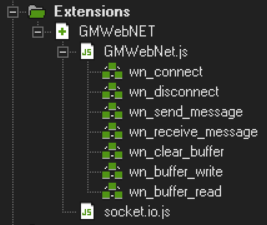
\includegraphics[scale=1.2]{images/extensions_folder.png}
\caption{View inside the GUI that visualises the extension function mapping setup.}
\label{fig:extension_folder}
\vspace{1em}
\end{figure}

\begin{figure}[H]
\centering
% \centering% default with `floatrow`
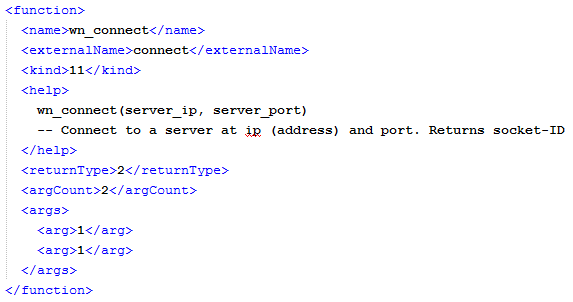
\includegraphics[scale=1.2]{images/xml_mapping.png}
\caption{External function \texttt{connect} from JavaScript extension file located in GMWebNet.js, mapped to a GML function \texttt{wn\_connect} located in the client application. The function takes 2 arguments, each of type String (id = 1), and returns a Double type (id = 2)}
\label{fig:xml_mapping}
\vspace{1em}
\end{figure}

The natively supported networking functions can easily be translated into the the browser-compatible functions defined by the extension as displayed in table \ref{table:function_translations}. The following purposes are included:
\begin{itemize}
\item initiating a connection
\item creating a packet in the buffer
\item sending a packet
\item spot incoming messages
\item read incoming messages
\item disconnect hosts
\end{itemize} 
\begin{center}
\begin{table}
  \begin{tabular}{ | l | }
  \hline
\textbf{Function Translations} \\

\hline
\textit{Creating a socket and connecting to a server}	\\
  \begin{tabular}{ l }
	\\ Native \\
	\texttt{socket = network\_create\_socket(network\_socket\_tcp);} \\
	\texttt{network\_connect(socket, ip\_address, port);} \\
	\\ Extension \\
	\texttt{socket = wn\_connect(ip\_address, port);}
  \end{tabular}
  \\\\
  
\hline
\textit{Creating a new packet in the buffer and sending it}	\\
  \begin{tabular}{ l }
	\\ Native \\
	\texttt{buffer = buffer\_create(size, type, byte\_alignment);} \\
	\texttt{buffer\_write(buffer, buffer\_size, value);} \\
	\texttt{network\_send\_packet(socket, buffer, buffer\_get\_size(buffer));} \\
	\\ Extension \\
	\texttt{wn\_buffer\_clear()} \\
	\texttt{wn\_buffer\_write(value)} \\
	\texttt{wn\_send\_message(socket)}
  \end{tabular}
  \\\\

\hline
\textit{Spot an incoming packet and start reading it}	\\
  \begin{tabular}{ l }
	\\ Native \\
	\texttt{new\_messages = socket\_read\_message(socket, buffer)} \\
	\texttt{if (new\_message) \{message = buffer\_read\_uint8(buffer);\}}\\
	\\ Extension \\
	\texttt{new\_messages = wn\_receive\_message(socket)} \\
	\texttt{if (new\_message) \{message = wn\_buffer\_read();\}}
  \end{tabular}
  \\\\

\hline
\textit{Disconnecting the hosts}	\\
  \begin{tabular}{ l }
	\\ Native \\
	\texttt{network\_destroy(socket);}\\
	\\ Extension \\
	\texttt{wn\_disconnect(socket, disconnect\_message\_id)}
  \end{tabular}
  \\\\

	\hline
  \end{tabular}
  \caption{Function Translations from natively supported functions to browser-supported functions. Notice that the extension itself takes care of implementation details for the buffer, buffer size and the connection type (TCP).}
  \label{table:function_translations}
  \end{table}
\end{center}


\section{Applications Developed with the Extension}
%Explain about ownmade application using the extension, how it tests the given benchmarks (eg. delay, data, equality)
\subsection{Benchmark Application}
The benchmark application was the first application created using the networking extension. It initially consisted of a single instance repeatedly sending a ping request to the server at a fixed interval, out of which the RTT could be calculated.

Since then, it has evolved into supporting a variety of instances (virtual clients), each being connected to the server through their own private connection. This way, it would allow for evaluation with many clients without being limited to a small amount of physical devices. The virtual clients are set to send messages at fixed intervals (ticks).

As the benchmarking application supports more than one virtual client that connects to the server, the benchmarker keeps track of the values of each of its virtual clients, calculating the averages, displaying these in a graph and creating logs for later evaluation.

On the top-left of the figure \ref{fig:benchmark_gui} the global data can be seen. This data only regards the virtual clients (not all clients that may be running on other devices). 

The \texttt{CPU} value indicates the speed at which the CPU processes the code at runtime. This had to remain at a steady 60 in order to ensure no external variabilities would interfere with the experiments. Similarly, the \texttt{FPS} had to remain at a steady 30fps. This was the frame rate at which the application is drawing the GUI. If at any point the CPU or FPS would drop, this would indicate an external factor is affecting the program execution and will potentially corrupt the test results. Therefore, values that were collected when these values dropped would automatically be discarded.

The \texttt{clients} variable indicates the number of virtual clients the application has created. 

\texttt{real\_clients} indicates the number of clients that have successfully established a private connection to the server.

\texttt{global\_clients} shows the user how many physical and virtual clients are connected to the server globally. This includes clients that are connected through other devices. This number is only updated on request by the user, as it depends on a request to the server and could reduce the accuracy of the experiments. Upon receiving this request, the server has to reply with the number of clients it is serving at that given time.

\texttt{average} and \texttt{deviation} refer to the average RTT and RTT deviation of the most recently sent 8-byte messages by each of the virtual clients.

\texttt{ping-rate/s} is the amount of 8-byte messages that are sent by each virtual client every second.

The \texttt{total req/sec} therefore indicates how many messages are sent out to the server every second by all of the virtual clients collectively.

\texttt{ping count} describes the size of the message history. 40 means that the graph will display the last 40 ticks worth of average RTTs of all the virtual clients.

This application was used in the evaluation experiments in order to test the system's capabilities, such as the applied stress on the server with different varieties of concurrent connections, certain amounts of messages that need to be processed simultaneously, as well as recording the effect on the RTT when the client is located in different areas in the world.

\begin{figure}
\centering
% \centering% default with `floatrow`
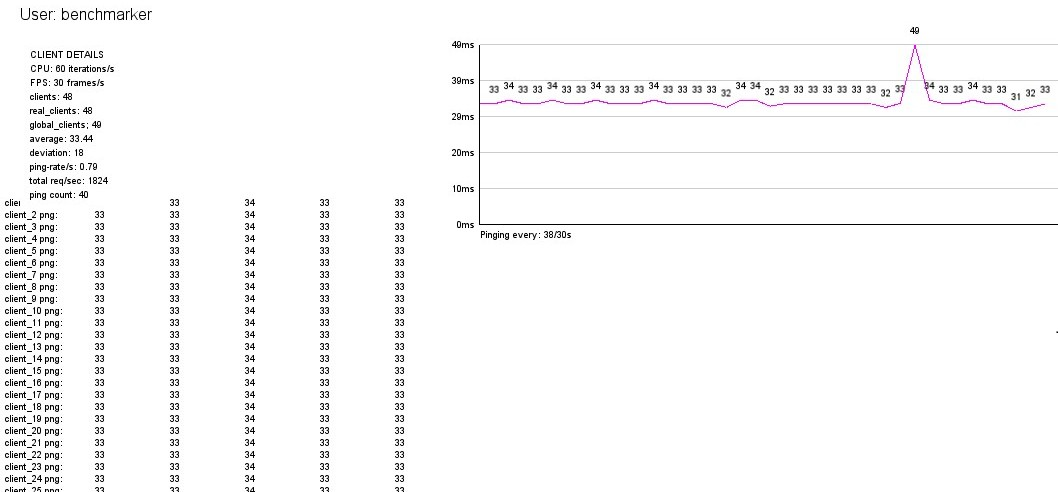
\includegraphics[scale=0.4]{images/benchmarker.jpg}
\caption{Displaying the GUI of the benchmarking application. On the left top the global data is available for the client. The table below displays the virtual clients and their 5 most recent roundtrip values. The graph on the top-right displays the average RTT over time for these clients. The colors of the image are inverted from the actual interface.}
\label{fig:benchmark_gui}
\vspace{1em}
\end{figure}

\subsection{Real Game Application}
\subsection{Developer Template}







% -----------------------
\chapter{Network Extension Evaluation}
%description of experiments, presentation + (directly including) interpretation of the data

\section{Controlled Network}
Controlled experiments were conducted in order allow prediction of server behaviour when loaded under similar pressure in future occasions.

Experiments were executed on a Windows 7 64-bit platform with 12.6GB available physical memory and an Intel(R) Core(TM) i7-2600K CPU @ 3.40GHz processor. The software entailed Node v0.12.3 and Socket.io v1.3.7 in order to handle the networking operations.

The network was controlled using Dummynet, using a below-average UK household network bandwidth \cite{household_bandwidth}. This involves an upload speed of 5Mbit/s, and a download speed of 1Mbit/, although no packet loss was set in order to ensure consistency throughout the controlled network experiments.

\subsection{Concurrent Connections}
It is important to know how many clients a server can host simultaneously. The following experiments evaluate the server performance in terms of server CPU usage, CPU time and RSS with regard to the number of concurrently connected clients.

\paragraph*{Setup}
\begin{itemize}
\item Variable number of concurrent connections cc, up to 15 instances with each simulating at most 500 clients.
\item Clients do \emph{not} contact the server after establishing a connection.
\item The resulting values are averaged over a 2-minute run duration.
\item After each run, the number of clients simultaneously connected to the server increases by 100.
\end{itemize}



\begin{figure}
\centering
% \centering% default with `floatrow`
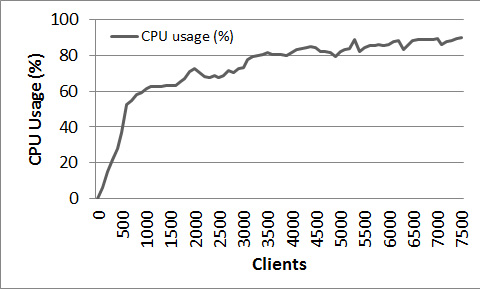
\includegraphics[scale=0.75]{images/test_CLIENT_CPUusage.jpg}
\caption{Displaying the CPU usage for the server process in percent.}
\label{fig:cpu_usage}
\vspace{1em}
\end{figure}

Figure \ref{fig:cpu_usage} indicates a logarithmic trend in the CPU usage on the server. When the CPU usage reaches over 80 percent, the user may experience lag. Such high CPU usage indicates insufficient processing power. Either the CPU needs to be upgraded, or the user experience reduced.

\begin{figure}
\centering
% \centering% default with `floatrow`
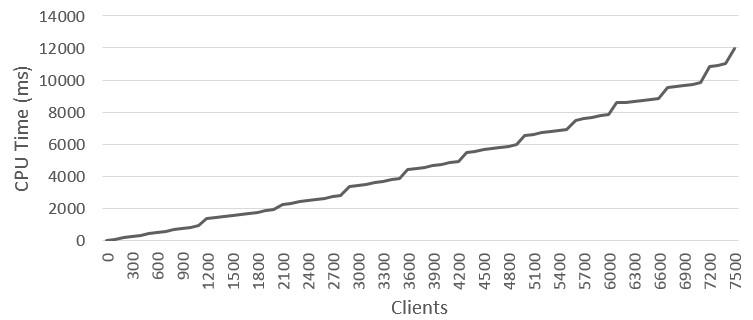
\includegraphics[scale=0.75]{images/test_CLIENT_CPUtime.jpg}
\caption{CPU time in milliseconds, displaying the amount of time required for the server to process the clients.}
\label{fig:cpu_time}
\end{figure}



\begin{figure}
\centering
% \centering% default with `floatrow`
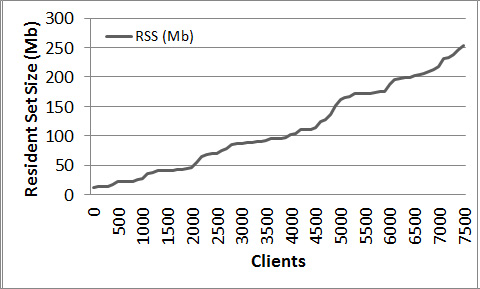
\includegraphics[scale=0.75]{images/test_CLIENT_RSS.jpg}
\caption{Resident set size in Megabit, showing the portion of RAM that is occupied by the server process.}
\label{fig:cpu_rss}
\end{figure}

Due to The server stores connection details for each client directly in the RAM.



\subsection{Message Broadcasting Performance}
The following experiment evaluates the number of messages that can be handled by the server simultaneously, and considers how this affects the fairness in response-time of the individual clients.

\paragraph*{Environment Setup}
\begin{itemize}
\item 5000 concurrent connections (10 instances each simulating at most 500 clients).
\item Each package that is sent has a size of 8 bytes.
\item Each client sends packages at regular time intervals, causing the server to handle n messages every second.
\item Each client measures the roundtrip time of its package to the server.
\end{itemize}

\paragraph*{Dependent variables}
\begin{itemize}
\item Mean roundtrip time between all clients
\item Variance of the roundtrip time between all clients
\item Standard Deviation of the roundtrip time between all clients
\end{itemize}

\begin{center}

\begin{figure}[h]
\centering
% \centering% default with `floatrow`
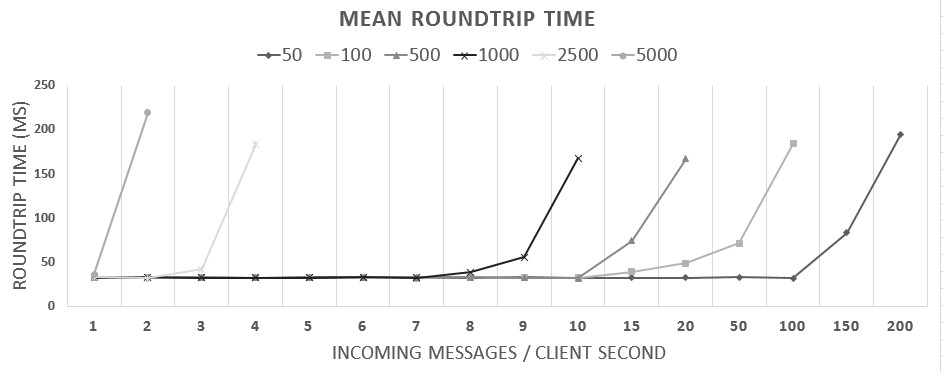
\includegraphics[scale=0.32]{images/test_SERVER_RTTmean.jpg}
\caption{The mean roundtrip time of all the messages that pass through the server. As expected, with few concurrent clients connected to the server, the server manages to broadcast many more messages.}
\label{fig:broadcast_rtt_mean}
\end{figure}



\begin{figure}
\centering
% \centering% default with `floatrow`
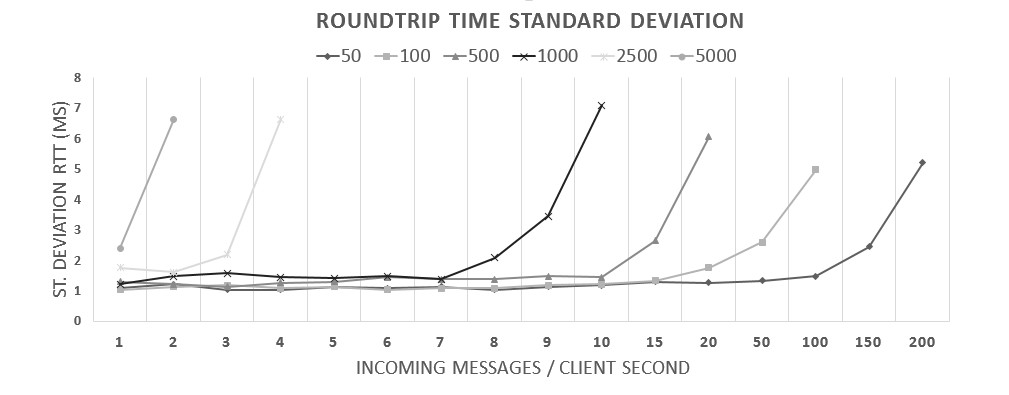
\includegraphics[scale=0.32]{images/test_SERVER_RTTstd.jpg}
\caption{Standard deviation of the message roundtrip times.}
\label{fig:broadcast_rtt_std}
\end{figure}

\end{center}



\section{Real Network Results}
The network was consistently running with a 54.0Mb/s download and 3.0Mb/s upload speed.
\paragraph*{}Multiple tests were executed with clients being located at specified locations. In each case, the clients were sending 8-byte messages to the server at a regular interval of 1 second for 2 minutes. The 120 roundtrip times for each client were then averaged in order to blur occasional peaks. At this point the roundtrip times of the clients in each common location were averaged, and then the deviance of the roundtrip times at each of these locations were calculated.

All network experiments were executed using a single server located in Edinburgh and in each experiment all clients were connected and communicating to that server simultaneously. During the experiments, logs were saved at the clients. After each experiment, these logs were forwarded for post-processing purposes. The roundtrip times represent the delay times between the packet-send event, and the packet-receive event by the same client for the same packet.

\subsection{Location-wise Delay Fairness}
The following experiment evaluates the effect of the geographical distance between groups of clients and the server with respect to fairness in response-time from the server to the clients.

\paragraph*{Test cases:}
\begin{enumerate}
\item Local network setting: Five clients physically located in the same local home network.

\item Same city: Five clients physically located in Edinburgh (LAN excluded).

\item Same country: Three clients physically located in Scotland: Edinburgh, Glasgow and Dundee.

\item Europe: Five clients physically located in the United Kingdom, Hungary, France, Germany and the Netherlands.

\item Inter-continental: Eight clients physically located in South Africa, California (USA), India, Thailand, Germany, Hungary, United Kingdom and the Netherlands.

\end{enumerate}

\paragraph*{Results:}Average roundtrip times per location:
\begin{center}
  \begin{tabular}{ r | l }
Location		& Average RTT \\ \hline\hline
LAN				& 32ms	\\
Edinburgh		& 55ms	\\
Dundee			& 65ms	\\
Germany			& 67ms	\\
Glasgow			& 68ms	\\
France			& 69ms	\\
the Netherlands	& 70ms	\\
United Kingdom	& 71ms	\\
Hungary			& 76ms	\\
India			& 103ms	\\
South Africa	& 144ms	\\
California (USA)& 158ms	\\
Thailand		& 171ms	\\
  \end{tabular}
\end{center}

Average roundtrip times per test:
\begin{center}
  \begin{tabular}{ | r || c | c | c | c | c |}
    \hline
    Test case 		& 1 		& 2 		& 3 		& 4 		& 5 		\\ \hline\hline
    Mean RTT 		& 32.1ms 	& 54.8ms 	& 62.7ms 	& 70.6ms 	& 107.5ms	\\ \hline
    Std RTT			& 0.4ms		& 2.9ms		& 6.8ms		& 3.36ms	& 43.6ms	\\ \hline
  \end{tabular}
\end{center}



% -----------------------
\chapter{Conclusion and Future Work}
\section{Conclusion}
\subsection{Comparison of the Extended GameMaker Functionality with Related Work}
\subsection{Criticism on the Implementation and Design Decisions}
%make clear connection with the evaluation
\section{Note to developers}
%Note: add reminder that developers can setup peer-to-peer network by using the extension to serve as both server and client in their client application, but that these tests specifically consider the strength of each individual application acting as server.

\section{Future Improvements}






% -----------------------
% >>>> REMOVE THIS BLOCK
\cite{Multiplayer_Networking_modern_engine} %unused
\cite{Fairness_and_Playability}
\cite{Pro_HTML5_Programming} %unused
\cite{HTML5_Up_and_Running}
\cite{Friendly_Programming} %unused
\cite{Mark_Overmars}
\cite{Death_Flash_Java}
\cite{Why_Nodejs}
\cite{Node_Stress_Test}
\cite{NodeJS_Image}
\cite{Socketio_Benchmark}
\cite{Socketio_TCP_Benchmark}
\cite{Socketio}
\cite{Canvas_API}
\cite{Web_Apps_Superior}
\cite{Community_Social_Psychology}
\cite{Why_MMOG} %unused
\cite{Browser_Games}
\cite{Browser_Networking}
\cite{Web_Apps_Superior}
\cite{P2P_Video_Streaming_HTML5_WebRTC}
\cite{Gamemaker_DnD}
\cite{GameMaker_Studio}
\cite{Optimizing_Multiplayer_3D_Game_Synch} %unused
\cite{Optimizing_WebSockets_Bandwidth} %unused
\cite{Google_Play_Store}
\cite{Apple_App_Store}
\cite{HTML5_Game_Dev_Gamemaker} %unused
\cite{SE_7_Principles}
\cite{Software_Engineering}
\cite{Construct2_Multiplayer_Tutorial}
\cite{WebSocket}
\cite{NAT}
\cite{Where_WebRTC}

\cite{handshake}
\cite{tcp_open_connection}
\cite{udp_connectionless}
\cite{udp_holepunching}
\cite{websocket_communication}
\cite{gamemaker_missing_networking}
\cite{gamemaker_networking_attempt}
\cite{yoyogames_forum}
\cite{dutch_gamemaker_forum}
\cite{html5_gamedev_tools}
\cite{html5_mozilla}
\cite{alexa_ranking}
\cite{gamepix_engines}
\cite{scirra_forum}
\cite{construct2_multiplayer}
\cite{unity_support}
\cite{unity_networking}
\cite{unity_websocket_sharp}
\cite{unity_forum}
\cite{unity_forum_2d}
\cite{unity_suggests_gamemaker}
\cite{github}
\cite{socketiojs}
\cite{household_bandwidth}


% <<<< REMOVE THIS BLOCK

%TODO change style to apa before submission. ignore "errors", it should still work after a few retries
\bibliographystyle{unsrt}
\bibliography{mybibfile}

\end{document}
